% !TEX TS-program = pdflatexmk
\documentclass[11pt]{article}
\usepackage[margin=1in]{geometry} 
\usepackage[parfill]{parskip}% Begin paragraphs with an empty line rather than an indent
\usepackage{graphicx}
\usepackage{booktabs}
%\pdfmapfile{=zi4.map}
%SetFonts
% inconsolata text
\usepackage[nott]{inconsolata}
\let\ttdefault\rmdefault
\usepackage[T1]{fontenc}
%\usepackage[scaled=.83]{beramono}
%\usepackage[varqu]{zi4}
%\usepackage{amsmath,amsthm}
\usepackage{newtxmath}
\usepackage{textcomp}
%\renewcommand\rmdefault{LinuxLibertineT-OsF}
%\usepackage[supstfm=libertinesups,%
%  supscaled=1.2,%
%  raised=-.13em]{superiors}
%SetFonts
%\UndeclareTextCommand{\textquotesingle}{LY1}
%\DeclareTextSymbol{\textquotesingle}{TS1}{39}
%\usepackage{upquote}
\title{The Inconsolata  Package}
\author{Michael Sharpe}
\date{\today}  % Activate to display a given date or no date

\begin{document}
%\show\textquotesingle
\maketitle
The package provides updated \emph{PostScript} and Opentype versions of Raph Levien's fine sans serif typewriter font
\texttt{Inconsolata} in regular and bold weights, adding some glyphs which may optionally replace existing \texttt{quotedbl} and \texttt{quotesingle} and lower-case~L, along with new slashed zero, \texttt{arrowright} and \texttt{arrowleft} glyphs. As of version 1.11,  narrower renditions are also provided, with widths reduced from 500 units to 450 units. \LaTeX\ support files are also provided for both. 

\section*{\LaTeX\ usage}
To use {\texttt{Inconsolata} as your typewriter font, add the line \verb|\usepackage{inconsolata}| (or, equivalently, \verb|\usepackage{zi4}|) to your preamble after any other packages that might load another typewriter font.  This
will change the typewriter font family to \texttt{zi4}, the family name used
by this package, which replaces the old \textsf{inconsolata}, where the family name was \texttt{fi4}.  (The original {\tt inconsolata} is now obsolete and is no longer distributed as part of \TeX Live.) 

As with Karl Berry's original \texttt{inconsolata} package, the new package offers four basic encodings---\texttt{T1}, \texttt{LY1}, \texttt{OT1} and \texttt{QX}---plus a \texttt{TS1} text companion encoding. It provides the following options which some may find improve its utility for displaying verbatim text such as code fragments. 
\begin{itemize}
\item With option {\bf nott}, the effect is to make {\tt zi4} the default Roman font rather than the default Typewriter font, turning on hyphenation and variable spacing. If this option is specified, it would be a good idea to choose a serifed Typewriter for the sake of contrast. As there are neither italics nor small caps available, you will need to find another way to emphasize small portions of text, and bold would seem to be the easiest to set.
(This document is typeset using this option.)
\item The option \textbf{scaled=x} (or \textbf{scale=x}) allows you to scale all typewriter text and verbatim text by the factor \textbf{x}.
\item
The default zero in \textbf{zi4} is now slashed. The unslashed zero may be specified with the option \textbf{var0}.
\item For those who find the default lower-case L(\texttt{l}) a bit too close to the numeral~\texttt{1}, there is an option \texttt{varl} which substitutes a more distinctive shape for all glyphs related to lower-case L.
\item The main package loads the \textbf{textcomp} package, which points to a TS$1$-encoded font that has been modified to have uncurved left and right quotes, especially important in code fragments, by use of \texttt{textcomp} glyphs \verb|\textasciigrave| and \verb|\textquotesingle|. The \textbf{varqu} option provides further upright quote forms for glyphs that are not part of the \texttt{textcomp} package, such as 
the default double quote glyph \texttt{quotedbl} and \texttt{quotesingle}, which by default have a small slant. (Note that the latter is not part of all encodings---it is present in \texttt{OT1}, \texttt{LY1} and \texttt{QX}, but not in \texttt{T1}.)
\item The package loads \texttt{upquote} by default, but provides an option \texttt{noupquote} to override it.
\item (new in v.1.11) The option \texttt{narrow} causes the narrow versions to be used, having widths reduced by 10\%.
\item (new in v.1.11) The default behavior of {\tt inconsolata} is to prevent all automatic hyphenation, to permit spacing to stretch and shrink, and to place some extra space after a line ending period. This version offers the following options to change the default behavior.  
\begin{itemize}
\item
Option \textbf{hyphenate} allows automatic hyphenation to occur, which may be useful if your usage is simply to have blocks of text in quasi-typewritten form, though with variable word-spacing.
\item option \textbf{mono} forces the behavior to mimic that of the Computer Modern Typewriter font---all spaces have the same width as the glyphs, and a full extra space is inserted after a line-ending period.
\item You may modify individual {\tt fontdimen} values that govern this behavior by means of the options \textbf{spacing}, \textbf{stretch}, {\tt shrink} and {\tt extrasp}. These will override any values changed by the option \textbf{mono}, for example, giving you a way to get monospacing but prevent extra space after a period, with
\begin{verbatim}
\usepackage[mono,extrasp=0em]{inconsolata}
\end{verbatim}
\end{itemize}
\end{itemize}
When used in ordinary typewriter mode (i.e., with \verb|\texttt{}| or the deprecated form \verb|{\tt }|), left and right quotes are rendered as in ordinary text. For example, 
\begin{verbatim}
\texttt{`xy' " \textasciigrave \textquotesingle}
\end{verbatim}
renders (with option \texttt{varqu}) as \texttt{`xy' " \textasciigrave \textquotesingle}. With the \texttt{upquote} package, verbatim text, eg:
\begin{verbatim}
\verb|`xy' "|
\end{verbatim}
 renders as you would expect it in code samples:
\verb|`xy' "|

\textbf{TeX Ligatures:} As of version {\tt 1.12}, text mode follows the usual TeX ligature rules with the exception of the f-ligatures, at least in T1 and LY1. Behavior on OT1 and QX encodings is limited to a subset of those rules. So, for example, in T1 and LY1:
\begin{center}
  \begin{tabular}{@{} cc @{}}
    \toprule
    Input & Output \\ 
    \midrule
    \verb|\texttt{a-b}| & a-b \\ %\texttt{a-b} \\ 
	\verb|\texttt{a--b}| & a--b\\ %\texttt{a--b} \\ 
	\verb|\texttt{a---b}| & a--b \\ %\texttt{a---b} \\
	\verb|\texttt{<<a>>}| & <<a>> \\ %\texttt{<<a>>} \\ 
    \verb|\texttt{?`}| & ?` \\ %\texttt{?`} \\ 
    \verb|\texttt{!`}| & !` \\ %\texttt{!`} \\ 
    \verb|\texttt{``}| & `` \\ %\texttt{``} \\ 
    \verb|\texttt{''}| & '' \\ %\texttt{''} \\ 
    \bottomrule
  \end{tabular}
\end{center}

Obviously, the distinctions between {\tt hyphen}, {\tt endash} and {\tt emdash} are subtle, as is to be expected given that  the glyphs are of fixed width.

\textbf{Note on the QX encoding:} The encoding files used as part of this package, derived from the \texttt{inconsolata} package, seem to have some inconsistencies with \texttt{qxenc.def} made necessary as a compromise to get text and verbatim modes functioning for a wide class of common characters.

In the following examples, the claim that all encodings render the same applies only to the very limited selection of quote glyphs tested. In practice, QX encoding behaves worse than the others for \texttt{inconsolata}/\texttt{zi4}.


\section*{Effects of the options varqu, noupquote}
\textbf{With \texttt{varqu}:} \texttt{upquote} loaded by default---all encodings render the same.

\begin{center}
  \begin{tabular}{@{} ccc @{}}
    \toprule
    Input & Text mode & Verbatim mode \\ 
    \midrule
    \verb|\textasciigrave| & \texttt{\textasciigrave} &   \\ 
    \verb|\textquotesingle| & \texttt{\textquotesingle}  &   \\ 
    \texttt{"} & \texttt{"}  & \verb|"|  \\ 
    \verb|'| & \texttt{'}  & \verb|'| \\ 
    \verb|`| & \texttt{`}  & \verb|`| \\ 
    \bottomrule
  \end{tabular}
\end{center}
\textbf{Without \texttt{varqu}:} \texttt{upquote} loaded by default---all encodings render the same.
\begin{center}
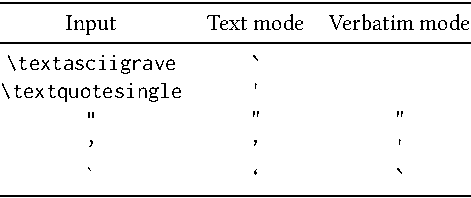
\includegraphics{novarqu-crop}
\end{center}
\textbf{Without \texttt{varqu}, \texttt{noupquote}:} \texttt{upquote} NOT loaded---all encodings render the same.
\begin{center}
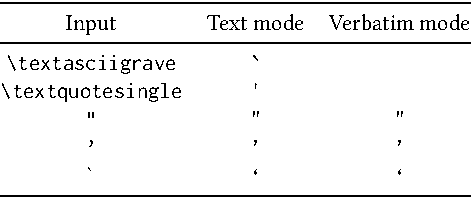
\includegraphics{novarqu-noupq-crop}
\end{center}
\textbf{With \texttt{varqu}, \texttt{noupquote}:} \texttt{upquote} NOT loaded---all encodings render the same.
\begin{center}
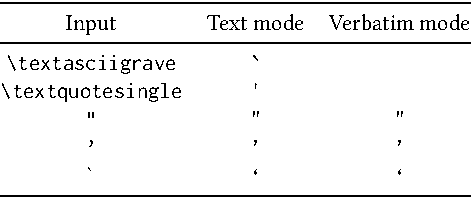
\includegraphics{novarqu-noupq-crop}
\end{center}


\textbf{Conclusion:} To me, it is overwhelmingly clear that the best results come from
specifying the option \texttt{varqu}, not specifying \texttt{noupquote}, and avoiding the QX encoding wherever  possible.

\textbf{A technical note concerning LY1 or QX encodings:} These encodings make their own definitions of \verb|\textquotesingle| as glyphs in the main text font. Using the TS1 glyph with upright shape so that \texttt{upquote} works correctly with these encodings requires the incantation:
\begin{verbatim}
\UndeclareTextCommand{\textquotesingle}{LY1} % or QX
\DeclareTextSymbol{\textquotesingle}{TS1}{39}
\usepackage{upquote}
\end{verbatim}
which is built-in to the \texttt{inconsolata.sty} (\textsc{aka} \texttt{zi4.sty})  code and need not be repeated.
\section*{Opentype issues} The package includes four Opentype fonts named \textsf{Inconsolatazi4-Regular}, \textsf{Inconsolatazi4-Bold}, \textsf{InconsolataN-Regular} and \textsf{InconsolataN-Bold}, the last two being for the narrow variant. The narrow and the normal width versions may be loaded using \texttt{fontspec}:
\begin{verbatim}
\fontspec{inconsolata} % normal width, slashed zero, curly quotes, default l
\fontspec{inconsolatan} % nnarrow width, slashed zero, curly quotes, default l
\end{verbatim}
The fonts contain three Stylistic Set variants that may be used to control the shape of lower case l (\texttt{ss01}), the form of zero (\texttt{ss02}) and the shape of quotes (\texttt{ss03}). One or more of these may be specified using one of the following example lines:
\begin{verbatim}
\setmonofont[StylisticSet=1]{Inconsolatazi4} % shapely l
\setmonofont[StylisticSet=2]{Inconsolatazi4} % unslashed zero
\setmonofont[StylisticSet=3]{Inconsolatazi4} % straight quotes
\setmonofont[StylisticSet={1,3}]{Inconsolatazi4} % shapely l, upright quotes
\end{verbatim}
To prevent automatic hyphenation, add the option {\tt HyphenChar=None} to the call. (Specifying {\tt inconsolata} as the font name tells {\tt fontspec} to look for the file {\tt inconsolata.fontspec} which spells out the names of the associated {\tt.otf} files.) 

Note that one cannot expect exactly the same rendition from \LaTeX\ typewriter modes and the \textsf{fontspec} typewriter modes. For one thing, in \LaTeX, the typewriter left quote symbol is \texttt{quoteleft}, while under \textsf{fontspec}, it is the \texttt{grave} symbol.
\end{document}



 